\documentclass[11pt,spanish,a4paper]{article}
% Versión 1er cuat 2014 Víctor Bettachini < bettachini@df.uba.ar >

\usepackage{babel}
\addto\shorthandsspanish{\spanishdeactivate{~<>}}
\usepackage[utf8]{inputenc}
\usepackage{float}
\usepackage{units}
\usepackage{siunitx}
\usepackage{amsmath}
\usepackage{amstext}
\usepackage{amssymb}
\usepackage{graphicx}
\graphicspath{ {./graphs/} {../}}

\voffset-3.5cm
\hoffset-3cm
\setlength{\textwidth}{17.5cm}
\setlength{\textheight}{27cm}

\usepackage{lastpage}
\usepackage{fancyhdr}
\pagestyle{fancyplain}
\fancyhead{}
\fancyfoot{}
\fancyfoot[C]{ {\tiny Actualizado al \today} }
\fancyfoot[RO, LE]{Pág. \thepage/\pageref{LastPage}}
\renewcommand{\headrulewidth}{0pt}
\renewcommand{\footrulewidth}{0pt}


\begin{document}
\begin{center}
	\textsc{\large Física 2 (Físicos)} - Prof. Hernán Grecco\\
	\textsc{\large Primer Cuatrimestre - 2014}\\
	\textsc{\large Guía 7:}	Ondas en más dimensiones
\end{center}

% - Para la primer práctica (7) agregar trazado de rayos. En el ej. 11, "haga trazado de rayos.
% Use fórmula del constructor de lentes"

\emph{LOS EJERCICIOS MARCADOS CON UN ASTERISCO (\textbf{*}) SON OPCIONALES}\\


\textbf{Propagación de ondas en medios / Ley de Snell-Sahl}

\begin{enumerate}
\item
\begin{enumerate}
	\item \textbf{*} Demostrar que para la ecuación de Klein-Gordon en tres dimensiones vale la relación de dispersión \(\omega^2= \omega_p^2 + v^2 k^2\).
	\item \textbf{*} Hallar las frecuencias típicas del plasma de la ionosfera, de los semiconductores y de los metales.
		Indicar la región del espectro electromagnético a la que pertenecen.
		¿Qué densidad de electrones haría falta para hacer un espejo para rayos X?
\end{enumerate}


\item \textbf{*} Demostrar que \(f(\hat{n} \vec{r} - ct)\) es solución de la ecuación de ondas clásica, donde \(\hat{n}\) es un versor constante en la dirección de propagación de la onda.


\item Una onda plana incide desde la izquierda (aire) sobre una lámina de vidrio de espesor \(e\), con un ángulo de incidencia \(\gamma\).
	Demuestre que la onda transmitida se propaga con el	mismo ángulo que la incidente.
	Escriba la expresión para:
	\begin{enumerate}
		\item la onda incidente en el sistema de referencia con origen \(O\) y eje \(z\); y con origen \(O\) y eje \(z\) según \(Z_1\).
		\item la onda reflejada, con origen \(O\) y eje \(z\); y con origen \(O\) y eje \(Z_2\).
		\item la onda transmitida dentro del material con origen \(O\); con origen \(O''\) y con \(O'''\).
		\item la onda transmitida con origen \(O'''\) y eje \(Z_4\); con origen \(O''\) y ejes \(Z_5\) y con eje \(z\).
		\item la onda reflejada en la segunda cara y transmitida hacia atrás en la primera, con origen \(O'\) y eje \(Z_3\) y con origen \(O\) y eje \(Z_2\).
	\end{enumerate}
	Analice los resultados y elabore una regla general sencilla para construir estas ondas.

    \begin{center}
		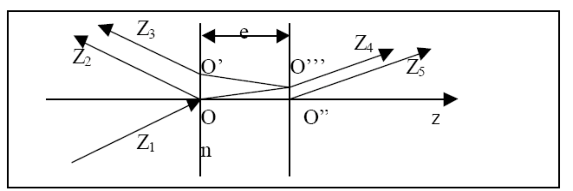
\includegraphics[width=0.55\linewidth]{g07e03}
	\end{center}


\item Una onda plana incide desde la izquierda perpendicularmente a la cara del prisma de la figura.
	Encuentre:
	\begin{enumerate}
		\item El ángulo de desviación \(\theta\) de la luz transmitida en función del índice de refracción y el ángulo \(\alpha\) del prisma.
		\item La dispersión del prisma (\(\mathrm{d}\theta/\mathrm{d}\delta\)).
			Estime dicho valor para algún material que encuentre en tablas o algún libro.
		\item El ángulo a partir del cual toda la luz es reflejada (ángulo de refracción rasante).
			Este ángulo se denomina de reflexión total interna.
			Discuta para qué caso es posible la reflexión total externa.
	\end{enumerate}
    \begin{center}
		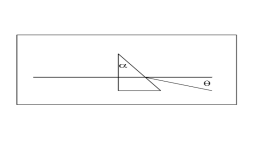
\includegraphics[width=0.35\linewidth]{g07e04}
	\end{center}


\item Para un vidrio los índices de refracción para el rojo y violeta son respectivamente \(1,51\) y  \(1,53\).
	Halle los ángulos de reflexión total para luz incidente en la superficie de separación aire-vidrio.
	Que ocurre si el vector de propagación de una luz blanca forma un ángulo de \(41^\circ\) con dicha superficie.


\item En un prisma con un ángulo de \(10^\circ\) incide luz roja y violeta.
	¿A que distancia de este debe ubicarse una pantalla para resolver (distanciar) estos colores en \SI{1}{mm}.


\item En las calmas y claras aguas del Caribe cubano (\(n \simeq 1.0003\)) un buzo suelda secciones de un oleoducto a \SI{80}{m} de profundidad.
	¿Hasta que distancia sus colegas en un bote podrán ubicarlo en la noche por sus luces?


\item \textbf{*} Demostrar que \(\Psi(x,t) = (A/r) \mathrm{e}^{i(k r- \omega t)} \) satisface la ecuación de Klein-Gordon y la de las ondas electromagnéticas en medios transparentes.
	Halle la relación de dispersión correspondiente.


\item  
\begin{enumerate}
	\item \textbf{*} Considere el frente esférico generado por una fuente puntual que emite en una longitud de onda (\( \lambda \)) y que se encuentra a una distancia \(d\) del punto de observación.
		¿Qué condiciones debe satisfacer \(\rho\) para que sea válida la aproximación paraxial?
	\item \textbf{*} Analice los siguientes casos: \(d= \SI{100}{\(\mu\) m}\); \SI{1}{cm}; \SI{1}{m}; \SI{100}{m} y \SI{10}{km}, con \(\lambda\) perteneciente a:
	\begin{enumerate}
		\item rango visible 
		\item microondas 
		\item onda corta
		\item rayos X
	\end{enumerate}
\end{enumerate}
	


\textbf{Lentes delgadas}

\item Escriba, en la aproximación paraxial, la expresión de una onda convergente a derecha a un punto \(P\).
	Halle la expresión de la onda reflejada en un espejo esférico de radio \(R_1\) en función de la distancia \(P\)-espejo.
	Discuta los distintos casos que se presentan.


\item \textbf{*} Halle la expresión de la onda transmitida cuando una onda esférica incide sobre una interfaz entre aire y vidrio, o dioptra, de forma esférica.


\item \label{eje} Se tiene una lente delgada en las condiciones que presenta la figura.
	Indique en qué punto del eje óptico debe incidir un rayo para que atraviese la lente sin desviarse. Exprese el resultado en función de la distancia focal objeto y de los índices de refracción.
	\begin{center}
		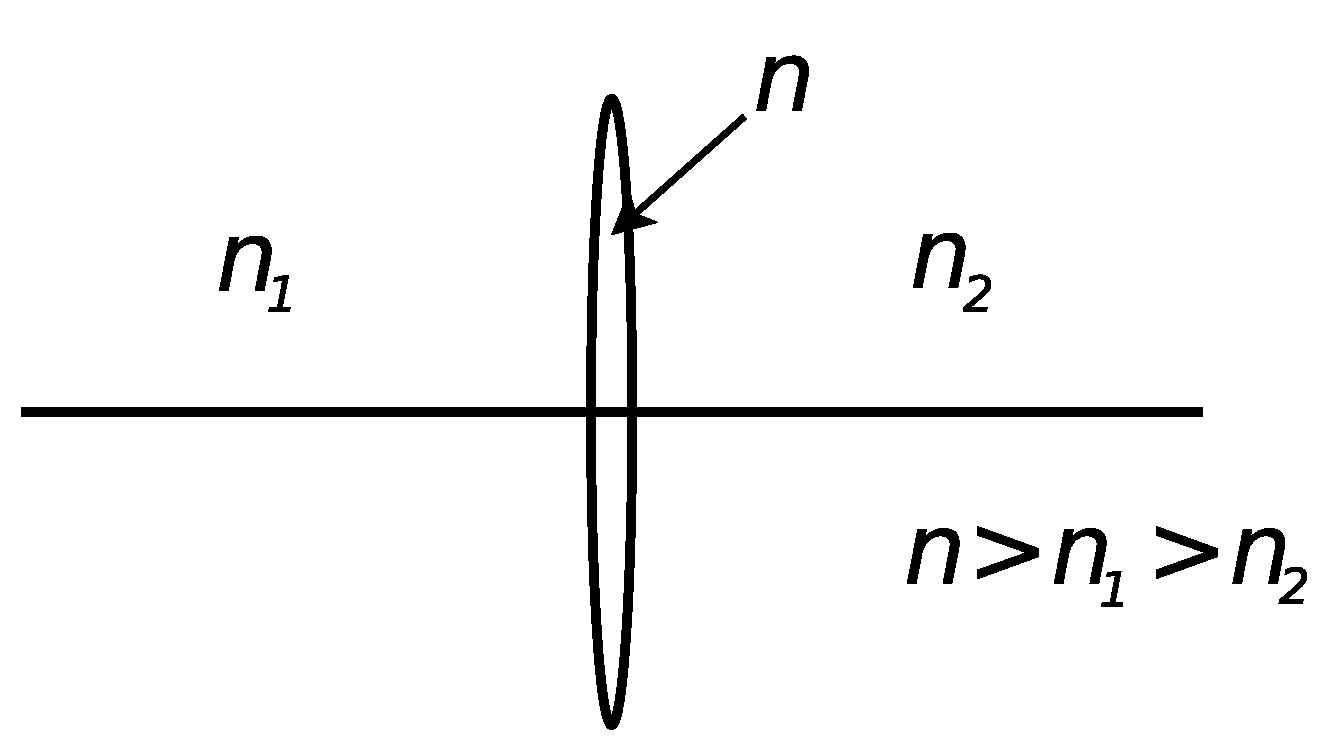
\includegraphics[width=0.25\linewidth]{ej3-25}
	\end{center}


\item \label{foco} Halle las distancias focales para lentes: i) plano-cóncava, ii) plano-convexa,
iii) bicóncava, iv) biconvexa, v) cóncava-convexa; en función del índice de refracción y
de los radios de curvatura de las lentes, como así también de los índices de refracción de
los medios externos.
En un caso particular demuestre que el resultado es independiente del orden en que se iluminan las superficies.


\item
\begin{enumerate}
	\item Defina qué se entiende por objetos e imágenes reales o virtuales.
		¿Cómo se generan y cómo se detectan?.
	\item \label{ant} Sea una fuente real a una distancia \(z_s\) de una lente de distancia focal imagen \(f'>0\).
		Para \(z_s> f\), \(z_s= f\) y \(z_s< f\), dibuje los frentes de onda incidentes y emergentes.
		Ídem. para \(f'< 0\).
	\item Ídem. \ref{ant} pero para una fuente virtual.
\end{enumerate}



\item \label{geom} Una lente forma imagen allí donde se crucen todos los vectores de propagación que la hayan atravesado.
	Basta con determinar el cruce de dos de estos para ubicar la imagen de un objeto.
	En particular un vector que pasa por un foco corresponde al otro lado de la lente con uno paralelo al eje de este.
	Así un rayo paralelo al eje de la lente desde un objeto tendrá su correspondiente pasando por el foco del lado opuesto (revisar ejercicio \ref{foco}).
	Si recordamos el resultado del ejercicio \ref{eje} tendremos el otro rayo que necesitamos. 
	Esta técnica geométrica de trazado de rayos es de mucha utilidad para corroborar resultados analíticos obtenidos con la ``fórmula del constructor de lentes''\footnote{Ecuación 7.7.12 en el libro \emph{Ondas es Física} de Martínez}.\\ \\
	Resuelva geométricamente a través del trazado de rayos, y determine si la imagen es real o virtual, es directa o invertida, para los siguientes casos:
	\begin{enumerate}
		\item Objeto puntual a \SI{20}{cm} de la lente de distancia focal \SI{10}{cm}.
		\item `` `` `` \SI{20}{cm} `` `` `` `` `` `` \SI{5}{cm}.
		\item `` `` `` \SI{3}{cm} `` `` `` `` `` `` \SI{5}{cm}.
		\item `` `` `` \SI{20}{cm} `` `` `` `` `` `` \SI{-40}{cm} (lente divergente).
	\end{enumerate}
	En todos los casos el objeto está a \SI{1}{cm} del eje de la lente.


\item Una adicta al tabaco sostiene frente a ella una ``lente de aire'' en la imagen de la izquierda.
	En los tres otros casos las lentes de vidrio tienen distintas curvaturas.
	Determine de que tipo son (convergentes/divergentes) y que clase de imagen (real/virtual) podemos ver de la futura ``cancerosa''.
	\begin{center}
		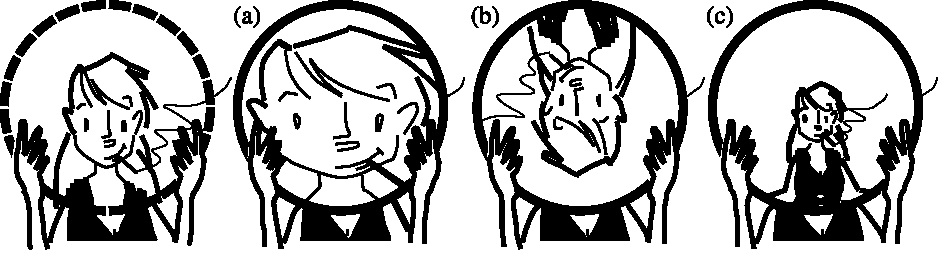
\includegraphics[width=0.75\linewidth]{fumadora}
	\end{center}


\item Ídem. el problema \ref{geom} pero ahora una lente delgada convergente, de distancia focal \SI{30}{cm}, se coloca \SI{20}{cm} a la izquierda de otra lente delgada divergente de distancia focal \SI{50}{cm}.
	    Para un objeto colocado a \SI{40}{cm} a la izquierda de la primera lente determine la imagen final.
		Determine además cuál es el aumento lateral del sistema.


	
\textbf{Dispositivos}


\item
\begin{enumerate}
	\item Describa el microscopio simple (lupa) y recordando que el aumento de un instrumento se define como el cociente entre el ángulo con que se ve al objeto a través del instrumento y el ángulo con que se lo ve a ojo desnudo, calcule su aumento en los siguientes dos casos:
	\begin{enumerate}
		\item imagen final en infinito, 
		\item imagen virtual a \SI{25}{cm} de la lupa.
	\end{enumerate}
	\item Describa un microscopio compuesto, enumerando cada uno de los elementos que lo componen y la función que cumple cada uno de ellos.
	Indique también si en la práctica cada uno de estos elementos es un elemento simple o no.
	¿Cómo se considera, a los efectos de resolución de esta guía, un microscopio compuesto?.
\end{enumerate}


\item Un microscopio consta de un objetivo de \SI{4}{mm} de distancia focal y de un ocular de \SI{30}{cm} de distancia focal.
	La distancia entre el foco imagen del objetivo y el foco objeto del ocular es \(g= \SI{18}{cm}\). Calcule:
\begin{enumerate}
	\item El aumento normal del microscopio, es decir el aumento cuando la imagen final está en el infinito.
	\item La distancia objeto-objetivo.
\end{enumerate}


\item Enumere los elementos básicos que componen un telescopio astronómico y los que componen un anteojo de Galileo, indique qué función cumple cada uno de ellos.
	Calcule el aumento de cada telescopio.


\item Un anteojo astronómico utiliza como objetivo una lente convergente de \SI{2}{m} de distancia focal y \SI{10}{cm} de diámetro, y como ocular una lente convergente de \SI{4}{cm} de distancia focal.
	Determine:
	\begin{enumerate}
		\item El aumento.
		\item El tamaño de la primera imagen de la luna y el tamaño angular de la imagen final a
través del telescopio.
La luna subtiende, a ojo desnudo, un ángulo de \SI{31}{'}.
	\end{enumerate}

	
\end{enumerate}
\end{document}
